\documentclass[14pt, master, substylefile = miee_master.rtx]{disser}

\usepackage[a4paper, includefoot, left=3cm, right=1cm, top=2cm, bottom=2cm, headsep=1cm, footskip=1cm]{geometry}

\usepackage[T2A]{fontenc}
\usepackage[utf8]{inputenc}
\usepackage[english, russian]{babel}
\usepackage{amsthm}

% Использовать полужирное начертание для векторов
\let\vec=\mathbf

% Включать подсекции в оглавление
\setcounter{tocdepth}{2}

\newtheorem{theorem}{Теорема}
\newtheorem{proposition}{Утверждение}
\newtheorem{lemma}{Лемма}

\begin{document}

\institution{Министерство образования и науки Российской Федерации \\ Федеральное агентство по образованию \\ Федеральное государственное автономное образовательное учреждение высшего образования <<Национальный исследовательский университет <<Московский институт электронной техники>> \\ Факультет Микроприборов и технической кибернетики \\ Кафедра высшей математики \textnumero 1
}

\apname{к.\,ф.-м.\,н., доцент А.\,А.~Прокофьев}

\title{Дисертация на соискание ученой степени магистра}

\topic{\normalfont\scshape %
<<?>>}

\author{Лебедев Михаил Евгеньевич}
\group{ВМ-22}

\sa {Г.\,Л.~Алфимов}
\sastatus{д.\,ф.-м.\,н., профессор}

\city{Москва}
\date{2016}

\maketitle

\tableofcontents

\intro

% TODO: разбавить научпопом
% TODO: совершенно не понятно, что такое FS и FGS
% TODO: разбавить Диминым дисером

Начиная с 90-х годов прошлого столетия, нелинейное уравнение Шредингера (НУШ) с дополнительной пространственной неавтономностью продолжает оставаться объектом пристального изучения.
Интерес к этому классу уравнений во многом обусловлен успехами в нелинейной оптики и исследованиям в области конденсата Бозе-Эйнштейна (БЭК).
БЭК --- это состояние вещества, возникающее при сверхнизких температурах, существование которого было предсказано в 20-е года XX века.
В 1995 г. БЭК был получен экспериментально \cite{Anderson}.
В настоящее время растущие экспериментальные возможности для получения и удержания этого нового состояния вещества ставят перед исследователями-теоретиками многочисленные вопросы, связанные как с объяснением имеющихся экспериментальных данных, так и с подготовкой новых экспериментов.
Оказалось, что динамика БЭК хорошо описывается уравнением шредингеровского типа с неавтономностью в виде дополнительного внешнего потенциала.
В контексте теории БЭК это уравнение носит название {\it уравнение Гросса-Питаевского}.
В дипломной работе рассматривается одномерный случай уравнения Гросса-Питаевского, которое имеет вид
%
\begin{equation}
i \Psi_t + \Psi_{xx} - U(x)\Psi + P(x)|\Psi|^2 \Psi = 0.
\label{eq:GPE}
\end{equation}
%
Здесь $\Psi(x, t)$ --- макроскопическая волновая функция конденсата, $U(x)$ соответствует потенциалу ловушки, удерживающей конденсат, а $P(x)$ описывает характерную длину межатомных взаимодействий частиц конденсата.
Используя явление так называемого резонанса Фешбаха, эта длина в эксперименте может быть сделана переменной, в частности изменяющейся периодически в пространстве \cite{Theis}.
Альтернативный подход основывается на использовании различных магнитных решеток, в которые погружается конденсат \cite{Jose}.
В этом случае говорят о взаимодействии конденсата с {\it нелинейной решеткой} (более подробно см. в обзоре \cite{Kartashov}).
Стоит отметить, что $P(x)$ может быть как знакопостоянной, так и знакопеременной функцией.
Особое внимание в литературе уделяется двум модельным случаям: $P(x) \equiv 1$ (случай межатомного притяжения) и $P(x) \equiv -1$ (случай межатомного отталкивания).
Величины
%
\begin{eqnarray}
&& E = \dfrac{1}{2} \int \Big( |\Psi_{x}|^2 + U(x) |\Psi|^2 - \dfrac{1}{2} P(x) |\Psi|^4 \Big) dx; \\ 
&& N = \int |\Psi|^2 dx,
\end{eqnarray}
%
имеют смысл энергии конденсата и числа частиц, образующих конденсат, соответственно.
Обе эти величины сохраняются при эволюции, описываемой уравнением (\ref{eq:GPE}).

Потенциал $U(x)$ в случае оптической ловушки также моделируется периодической функцией.
В этом случае говорят о {\it линейной решетке}, удерживающей конденсат.
Обсуждение соответствующих физических принципов можно найти в работе \cite{Pitaevskii}, а обзор результатов исследования уравнения Гросса-Питаевского с периодическим (линейным) потенциалом --- в работе \citep{Brazhnyi}.
В дальнейшем мы будем называть функцию $U(x)$ {\it линейным потенциалом}, а функцию $P(x)$ --- {\it нелинейным потенциалом}.

Стоит отметить, что уравнение (\ref{eq:GPE}) является широко востребованным в самых разных областях физики.
В оптике уравнение (\ref{eq:GPE}) описывает распространение света в планарных волноводах.
Пространственная модуляция в этом случае достигается за счет присадок неоднородной плотности, встроенных в волновод и усиливающих нелинейные свойства.
Таким образом, описание и исследование решений уравнения (\ref{eq:GPE}) для различных $U(x)$, $P(x)$ является актуальной математической задачей.

При исследовании задач, приводящих к уравнению (\ref{eq:GPE}), с физической точки зрения важную роль играют так называемые {\it стационарные моды}.
Им соответствуют решения вида $\Psi(x, t) = u(x) e^{-i \omega t}$.
Если $u(x)$ --- действительная функция, она удовлетворяет обыкновенному дифференциальному уравнению
%
\begin{equation}
u_{xx} + Q(x)u + P(x)u^3 = 0,
\label{eq:stationary}
\end{equation}
%
где $Q(x) = \omega - U(x)$.
Естественным (опять же с физической точки зрения) является {\it условие локализации} стационарной моды
%
\begin{equation}
\lim \limits_{x \to \pm \infty} u(x) = 0.
\label{eq:localization}
\end{equation}
%
Вместе с тем в литературе рассматриваются и другие типы стационарных мод, в частности, пространственно периодические и квазипериодические структуры.
Однако большая часть литературы посвящена именно стационарным решениям.
При этом внимание зачастую уделяется лишь простейшим видам локализованных стационарных мод, в частности так называемым {\it основным} стационарным модам, которые в англоязычной литературе носят название {\it fundamental solitons} (FS) или {\it fundamental gap solitons} (FGS).
Такие стационарные состояния минимизируют функционал энергии при заданном числе частиц, именно поэтому они и привлекают особое внимание в \cite{Kartashov}.
Рассмотрение {\it высших} (т.е. не являющихся основными) стационарных состояний также представляет интерес.
К примеру, они возникают в задачах по <<квантовому запутыванию>> различных конденсатов.

Второе важное условие, которое естественно потребовать от стационарные моды, это ее устойчивость.
Это означает, что достаточное малые возмущения стационарной моды не возрастают со временем.
Удовлетворение этому требованию важно для физических приложений, поскольку зачастую только устойчивые решения могут быть обнаружены в эксперименте и в дальнейшем использованы на практике.
Одной из глобальных задач, связанных с уравнением Гросса-Питаевского, является поиск и классификация новых локализованных стационарных мод и исследование их устойчивости.

Для описания множества стационарных мод необходимо детальное исследование множества решений уравнения (\ref{eq:stationary}).
Попытка такого исследования в случае, когда $P(x) \equiv -1$ (отталкивающие межатомные взаимодействия) и $Q(x)$ --- ограниченная периодическая функция, была сделана в работе \cite{AlfAvr}.
Основная идея работы \cite{AlfAvr} заключалась в том, что <<большая часть>> решений уравнения (\ref{eq:stationary}) уходит на бесконечность в некоторой конечной точке числовой прямой.
Далее, оказалось, что множество <<оставшихся>> решений, определенных на всей числовой прямой, при некоторых условиях можно полностью описать, используя методы символической динамики.
Более точно, эти решения могут быть поставлены во взаимно-однозначное соответствие с бесконечными в обе стороны последовательностями из символов некоторого конечного алфавита ({\it кодами} решений).
Из этого множества кодов можно выделить коды, соответствующие локализованным или периодическим решениям.
В работе \cite{AlfAvr} был проведен детальный анализ случая
$$Q(x) = \omega - A \cos 2x,$$
и была указана область на плоскости параметров $(\omega, A)$, где все определенные на всей числовой прямой решения можно закодировать бесконечными последовательностями из символов <<$0$>>,  <<$+$>>, <<$-$>>.
Локализованным модам при этом соответствуют коды, которые содержат лишь конечное число ненулевых символов.

Задачей, которая решается в ходе дипломной работы, является применение аналогичного подхода для случая, когда функция $P(x)$ является знакопеременной.
В частности, интересно посмотреть простейший случай периодической модуляции, когда $P(x) = \alpha + \cos 2x$, а $U(x) \equiv 0$.
Этот случай уже обсуждался в литературе (см. работу \cite{Malomed}) при рассмотрении солитонов в оптических решетках.
В ней подробно исследовалась устойчивость простейшего класса стационарных мод --- FS решений, и была показана устойчивость FS для большинства значений параметров.
Будет полезным подтвердить основные результаты этой работы и несколько расширить их.
В заключении вводной части резюмируем основные направления исследований.

\paragraph{Цели дипломной работы.}
\begin{itemize}
\item[1.] Обобщение результатов работы \cite{AlfAvr} на более широкий класс функций $Q(x)$, $P(x)$.
\item[2.] Поиск и разработка универсальных методов определения устойчивости стационарных мод.
\item[3.] Применение этих техник при рассмотрении модельного случая уравнения (\ref{eq:GPE}), когда $U(x) \equiv 0$, $P(x) = \alpha + \cos 2x$; поиск новых локализованных решений и исследование их устойчивости.
\end{itemize}
\chapter{Регулярные и сингулярные решения}

В этой главе представлены некоторые результаты аналитического исследования уравнения (\ref{eq:stationary}) для стационарных состояний.
Для дальнейшего условимся о следующей терминологии.
Решение $u(x)$ уравнения (\ref{eq:stationary}) будем называть {\it сингулярным}, если для некоторой конечной точки $x_0 \in \mathbb{R}$ выполняется соотношение
%
$$\lim \limits_{x \to x_0} u(x) = \infty.$$
%
При этом мы будем говорить, что решение $u(x)$ {\it коллапсирует} в точке $x_0$.
Соответственно, решение $u(x)$ уравнения (\ref{eq:stationary}), не коллапсирующее ни в какой точке $\mathbb{R}$, будем называть {\it несингулярным} или {\it регулярным}.

\section{$P(x) > 0$: отсутствие сингулярных решений}

В случае, когда $P(x)$ --- положительная функция, при некоторых других ограничениях оказывается справедливым следующее утверждение.

\begin{proposition}
Пусть $\forall x \in \mathbb{R}$, функции $Q(x), P(x) \in C^1(\mathbb{R})$, причем
%
\begin{itemize}
\item[(a)] $P(x) \ge P_0 > 0$, $|P'(x)| \le \widetilde{P};$
\item[(б)] $Q(x) \ge Q_0$, $|Q'(x)| \le \widetilde{Q};$
\end{itemize}
%
тогда решение задачи Коши для уравнения (\ref{eq:stationary}) с произвольными начальными условиями $u(x_0) = u_0$, $u_x(x_0) = u_0'$ может быть продолжено на всю действительную ось $\mathbb{R}$.
\label{prop:continuation}
\end{proposition}
%
\begin{proof}
По теореме существования решений для ОДУ, существует такой интервал $\Delta = [x_0; x_1)$, что решение задачи Коши $u(x)$ уравнения (\ref{eq:stationary}) с начальными условиями $u(x_0) = u_0$, $u_x(x_0) = u_0'$ на нем существует, единственно и $u(x) \in C^2(\Delta)$.
Предположим, что $[x_0; x_1)$ --- это максимальный интервал существования решения, т.е. решение задачи Коши не может быть продолжено за точку $x = x_1$.
Умножив исходное уравнение на $4u_x$ и проинтегрировав в пределах $[x_0; x)]$, $x < x_1$, получим
%
\begin{eqnarray}
2u_{x}^2(x) + 2Q(x)u^2(x) - 2{\int \limits_{x_0}^x Q'(\xi)u^2(\xi)d\xi} + P(x)u^4(x) - \\
\nonumber - {\int \limits_{x_0}^x P'(\xi)u^4(\xi)d\xi} = 2(u_0')^2 + 2Q(x_0)u_0^2 + P(x_0)u_0^4 \equiv C,\label{eq:integrated}
\end{eqnarray}
%
Где $C$ --- некоторая известная постоянная.
Отбрасывая $u_x^2(x) \ge 0$ в левой части равенства, а также пользуясь ограниченностью снизу функций $Q(x)$ и $P(x)$ значениями $Q_0$ и $P_0$ соответственно, приходим к неравенству
%
\begin{equation}
2Q_0 u^2(x) + P_0 u^4(x) \le C + 2{\int \limits_{x_0}^x
Q'(\xi)u^2(\xi)d\xi} + {\int \limits_{x_0}^x P'(\xi)u^4(\xi)d\xi}.
\label{eq:bound}
\end{equation}
%
Производные $Q'(\xi)$ и $P'(\xi)$ заменим их оценками сверху: $Q'(\xi) \le \widetilde{Q}$, $P'(\xi) \le \widetilde{P}$, где $\widetilde{Q} \ge 0$, $\widetilde{P} \ge 0$.
Умножив обе части неравенства на $P_0 > 0$, получим, что
%
\begin{equation}
2Q_0 P_0 u^2(x) + P_0^2 u^4(x) \le P_0 C + 2P_0 \widetilde{Q}{\int\limits_{x_0}^x u^2(\xi)d\xi} + P_0 \widetilde{P}{\int \limits_{x_0}^x u^4(\xi)d\xi}.
\end{equation}
%
Обозначим $v(x) = (P_0 u^2(x) + Q_0)^2$, $v(x) \ge 0$.
Тогда
%
\begin{equation}
v(x) \le \widetilde{C} +  \dfrac{\widetilde{P}}{P_0}\int \limits_{x_0}^x w(v(\xi))~d\xi. \label{eq:tov}
\end{equation}
%
Здесь $\widetilde{C} = P_0 C + Q_0^2 \ge 0$, $\alpha = {2\widetilde{Q} P_0}/{\widetilde{P}} \ge 0$, а $w(v)$ определяется формулой
%
\begin{equation}
w(v)\equiv\alpha (\sqrt{v} - Q_0) + (\sqrt{v} - Q_0)^2.
\label{eq:defw}
\end{equation}
%
Введем в рассмотрение функцию
%
\begin{equation}
G(s) = \int \limits_{s_0}^s \dfrac{dv}{w(v)}.
\label{eq:G}
\end{equation}
%
Здесь $s_0 \ge Q_0^2$ --- произвольная постоянная, $s \ge s_0$.
Так как $w(v)$ положительна и монотонно возрастает, а интеграл
%
\begin{equation}
\int \limits_{s_0}^{+\infty} \dfrac{dv}{w(v)}
\end{equation}
%
расходится, функция $G(s)$ является положительной, монотонно возрастающей и неограниченной.
Это означает, что обратная функция $G^{-1}(r)$ определена при $r \ge 0$, монотонно возрастает и неограничена.
Сказанное позволяет применить к (\ref{eq:tov}) неравенство Бихари, \cite{Pachpatte}, Теорема 2.3.1, из которого следует, что
%
\begin{equation}
v(x) \le G^{-1} \left( G(\widetilde{C}) +  \dfrac{\widetilde{P}}{P_0} {\int \limits_{x_0}^{x} d\xi} \right) = G^{-1} \left( G(\widetilde{C}) + \dfrac{\widetilde{P}}{P_0}(x - x_0) \right) < \infty.
\label{eq:bihari}
\end{equation}
%
Неравенство (\ref{eq:bihari}) справедливо при всех $x \in [x_0, x_1)$.
Таким образом, из (\ref{eq:bihari}) следует ограниченность функции $v(x)$ на всем промежутке $[x_0; x_1)$, а именно
%
\begin{equation}
v(x) \le M = G^{-1} \left( G(\widetilde{C}) + \dfrac{\widetilde{P}}{P_0}(x_1 - x_0) \right).
\end{equation}
%
Заметим, что $\widetilde{C} \ge Q_0^2$, причем $\widetilde{C} = Q_0^2$ только при $u_0 = u_0' = 0$.
Это означает, что $G(s)$ определена в точке $\widetilde{C}$ для любого ненулевого решения $u(x)$.
Из ограниченности $v(x)$ следует, что решение $u(x)$ также является ограниченным на всем промежутке $[x_0; x_1)$:
%
\begin{equation}
|u(x)| \le \sqrt{\dfrac{\sqrt{M} - Q_0}{P_0}},~x \in [x_0, x_1).
\label{eq:estimstion}
\end{equation}
%
Подставляя оценку (\ref{eq:estimstion}) в равенство (\ref{eq:integrated}), получаем оценку сверху для производной $u_x(x)$, справедливую на полуинтервале $x \in [x_0; x_1)$.
Поскольку функции $u(x)$ и $u_x(x)$ непрерывны и ограничены на $[x_0; x_1)$, значения $u(x_1)$ и $u_x(x_1)$ конечны.
Следовательно, существует продолжение решения задачи Коши с начальными условиями $u(x_0)$, $u_x(x_0)$ на интервал, больший чем $[x_0; x_1)$, что противоречит исходному предположению.

Таким образом, доказана возможность продолжения решения на всю полупрямую $x > x_0$.
Для доказательства аналогичного факта для $x < x_0$ достаточно сделать замену $x \to -x$ и повторить вышеизложенные рассуждения.
\end{proof}

Таким образом, в случае $P(x) > 0$ показано отсутствие сингулярных решений уравнения (\ref{eq:stationary}).
Из доказательства предложения \ref{prop:continuation}, в частности, следует, что если условия (а) и (б) выполняются не на всей числовой прямой, а только на некотором промежутке $[x_1;x_2]$, решение задачи Коши для уравнения (\ref{eq:stationary}) с произвольными начальными условиями не коллапсирует ни в какой точке промежутка $[x_1;x_2]$.

\section{$P(x) < 0$, $Q(x) < 0$: все решения сингулярны}

Для дальнейших рассуждений нам понадобится несколько вспомогательных лемм.

\begin{lemma}
Все решения уравнения
%
\begin{equation}
v_{xx} - qv - pv^3 = 0,
\label{eq:singular}
\end{equation}
%
где $p,q > 0$ --- постоянные, сингулярны, за исключением нулевого решения.
\label{lemma:singular}
\end{lemma}
%
\begin{proof}
Решение задачи Коши для уравнения (\ref{eq:singular}) с начальными условиями $v(x_0) = v_0$, $v_x(x_0) = v_0'$ может быть записано в неявном виде
%
\begin{eqnarray}
&&\pm {\int \limits_{v_0}^{v} \dfrac{d\xi}{\sqrt{C + q{\xi}^2 + \dfrac{p}{2}{\xi}^4}}} = x - x_0; \\
&& \nonumber C = (v_0')^2 - qv_0^2 - \dfrac{p}{2}v_0^4,
\end{eqnarray}
%
(выбор знака в левой части зависит от начальных условий и значения $x$).
Интеграл в левой части равенства сходится при $v \to \infty$, а значит, существует такое значение $x$,
%
\begin{equation}
x_{collapse} = x_0 + {\int \limits_{v_0}^{\infty} \dfrac{d\xi}{\sqrt{C + q{\xi}^2 + \dfrac{p}{2}{\xi}^4}}},
\end{equation}
%
при приближении к которому $v(x)$ стремится к бесконечности.
\end{proof}

Вторая лемма, которая понадобится нам для доказательства основного утверждения этого раздела, это так называемая лемма о сравнении (Comparison Lemma) из работы \cite{AlfZez}.
Она формулируется следующим образом.

\begin{lemma}[О сравнении]
Пусть функции $u(x)$, $v(x)$, $x \in [a; b]$ являются решениями уравнений
%
\begin{eqnarray}
&& u_{xx} - g(x, u) = 0; \\
&& v_{xx} - f(x, v) = 0,
\end{eqnarray}
%
соответственно.
Пусть также выполняются следующие условия:
\begin{itemize}
\item[(а)] $f(x, \xi)$, $g(x, \xi)$ определены на $[a; b] \times [A; B]$ и для них выполняется локальное Липшица по переменной $\xi \in [A; B]$ ($A$, $B$, $b$ могут быть как конечными так и бесконечными);
\item[(б)] $g(x, \xi) \ge f(x, \xi)$ для всех $x \in [a; b]$, $\xi \in [A; B]$;
\item[(в)] $f(x, \xi)$ монотонная, неубывающая по $\xi \in [A; B]$ функция.
\end{itemize}
Далее, пусть $A < v(a) \le u(a) < B$ и $v_x(a) \le u_x(a)$, тогда верно, что $v(x) \le u(x)$ и $v_x(x) \le u_x(x)$, пока выполняется $A < v(x), u(x) < B$, или же на всем интервале $x \in [a; b]$ (если $\forall x \in [a; b]$ $A < v(x), u(x) < B$).
\label{lemma:comparison}
\end{lemma}

Теперь все готово для доказательства следующего утверждения.

\begin{proposition}
Пусть при любом $x \in \mathbb{R}$ выполняются условия $P(x) \le P_0 < 0$, $Q(x) \le Q_0 < 0$, тогда  все решения уравнения (\ref{eq:stationary}) сингулярны, за исключением нулевого решения.
\label{prop:singular}
\end{proposition}
%
\begin{proof}
Используем Лемму \ref{lemma:comparison} о сравнении.
Рассмотрим уравнение
%
\begin{equation}
v_{xx} + Q_0 v + P_0 v^3 = 0.
\end{equation}
%
Введем следующие обозначения:
%
\begin{eqnarray}
&& g(x, \xi) = -Q(x)\xi - P(x)\xi^3;\\
&& f(x, \xi) = f(\xi) = -Q_0 \xi - P_0 \xi^3.
\end{eqnarray}
%
Применим Лемму \ref{lemma:comparison} о сравнении к паре уравнений
%
\begin{eqnarray}
u_{xx} - g(x, u) = 0; \label{eq:less} \\
v_{xx} - f(x, v) = 0. \label{eq:greater}
\end{eqnarray}
%

В области $D_+ = \{ x \in \mathbb{R},~\xi \in (0; +\infty) \}$ имеем $f(x, \xi) \le g(x, \xi)$. Пусть $\tilde{u}(x)$ --- решение задачи Коши для уравнения (\ref{eq:less}) с начальными условиями $u(x_0) = u_0$, $u'(x_0) = u_0'$.
Выберем начальные условия задачи Коши для уравнения (\ref{eq:greater}): $v(x_0) = u(x_0) = u_0$, $v'(x_0) = u'(x_0) = u_0'$; $\tilde{v}(x)$ -- ее решение.
Пусть $u_0 > 0$, тогда возможны два случая:

(а) $u_0' \ge 0$.
Функция $\tilde{v}(x)$  монотонно возрастает (этот факт легко установить из фазового портрета уравнения (\ref{eq:greater})).
Исходя из леммы о сравнении, решение $\tilde{u}(x)$ ограничивает сверху решение $\tilde{v}(x)$, которое, в свою очередь, сингулярно.
Следовательно, решение $\tilde{u}(x)$ также является сингулярным.

(б) $u_0' < 0$.
Сделаем замену $\tilde{x} = -x$.
В этом случае решение $\tilde{v}(\tilde{x})$  также монотонно возрастает, а, исходя из леммы
о сравнении, $\tilde{u}(\tilde{x})$ ограничивает его сверху, следовательно, является сингулярным.

Аналогично, в области $D_- = \{x \in \mathbb{R}, \xi \in (-\infty; 0)\}$ справедливо неравенство $f(x,\xi) \ge g(x,\xi)$.
Путем аналогичных рассуждений устанавливается, что в области $D_-$ решение $u(x)$ также будет сингулярным.
\end{proof}

\section{$P(x)$ не знакоопределена}

Если $P(x)$ отрицательна хотя бы в одной точке $x_0 \in \mathbb{R}$, формальные асимптотические разложения предсказывают существование {\it двух однопараметрических семейств решений} уравнение (\ref{eq:stationary}), коллапсирующих в этой точке.

\subsection{Асимптотика сингулярных решений}

Построим эти асимптотические разложения.
Будем считать, что $P(x_0)=-1$ (выполнения этого условия можно добиться путем перенормировки независимой переменной), введем обозначение $\eta = x - x_0$ и предположим, что в окрестности точки $x = x_0$ справедливы разложения
%
\begin{eqnarray}
&& Q(x) = Q_0 + Q_1 \eta + Q_2 \eta^2 + \dots; \\
&& P(x) = -1 + P_1 \eta + P_2 \eta^2 + \dots.
\end{eqnarray}
%
Имеем
%
\begin{equation}
u_{\eta\eta} + (Q_0 + Q_1 \eta + Q_2 \eta^2 + \dots)u + (-1 + P_1 \eta + P_2 \eta^2 + \dots)u^3 = 0.
\end{equation}
%
Коллапсирующие в точке $x = x_0$ решения этого уравнения удовлетворяют условию $u(\eta) \to \pm \infty$, $\eta \to 0$.
Пусть $\eta$ стремиться к нулю {\it справа}, $\eta > 0$.
Сделаем замены $v(\eta) = \eta u(\eta)$, $\eta = e^{-t}$.
Получим
%
\begin{equation}
v_{tt} + 3v_t + 2v + e^{-2t}Q(t)v + P(t)v^3 = 0.
\label{eq:collapse_asympt}
\end{equation}
%
Главный член разложения определим, исходя из баланса членов при $2v$ и $-v^3$.
Соответственно имеем
%
\begin{equation}
V_0(t) = \pm \sqrt{2}.
\label{eq:V0}
\end{equation}
%
Найдем первую поправку к главному члену, $v(t) = \pm \sqrt{2} + V_1(t) + o(V_1(t))$.
Подставляя последнее выражение в уравнение (\ref{eq:collapse_asympt}), учитывая разложение для функций $Q(t)$, $P(t)$ и отбрасывая члены порядков, более высоких, чем $e^{-t}$, получаем
%
\begin{equation}
V_{1,tt} + 3V_{1,t} - 4V_1 = \mp 2 \sqrt{2} e^{-t},
\end{equation}
%
откуда $V_1(t) = \pm \frac{\sqrt{2}}{3} e^{-t}$.
Вторая, третья и четвертая поправки, $V_n$, $n = 2,3,4$, находятся аналогичным образом.
Для каждой из них соответствующее уравнение принимает вид
%
\begin{equation}
V_{n,tt} + 3V_{n,t} - 4V_n = C_n e^{-nt}.
\label{eq:Vn}
\end{equation}
%
Однако, если при $n = 2,3$ решения уравнения (\ref{eq:Vn}) имеют вид $V_n \sim e^{-nt}$, то в случае $n = 4$ показатель экспоненты в правой части совпадает с одним из корней характеристического многочлена для оператора, стоящего в правой части.
В этом случае решение уравнения (\ref{eq:Vn}) необходимо искать в виде $Ce^{-4t} - A_3 t e^{-4t}$.
Здесь постоянная $C$ может быть выбрана произвольным образом, а $A_3$ однозначно определяется коэффициентами разложений для $Q(t)$, $P(t)$.
Если константа $C$ фиксирована, на дальнейших шагах указанной процедуры соответствующие уравнения разрешаются однозначно.
Отметим, что замена <<$+$>> на <<$-$>> в соотношении (\ref{eq:V0}) приводит к замене знаков на противоположные у всех коэффициентов $A_n$, $n = 0, 1, \dots$, что естественно в силу инвариантности уравнения (\ref{eq:stationary}) относительно замены $u \to -u$.
Получаем
%
\begin{equation}
\pm v(t) = \sqrt{2} + A_0 e^{-t} + A_1 e^{-2t} + A_2 e^{-3t} + A_3 \cdot (-t) \cdot e^{-4t} + Ce^{-4t} + \dots
\end{equation}
%
Явные выражения для $A_0, \dots, A_3$ таковы:
%
\begin{eqnarray}
&& A_0 = \dfrac{\sqrt{2}}{3} P_1; \label{eq:A_0} \\
&& A_1 = \dfrac{\sqrt{2}}{3} P_2 + \dfrac{\sqrt{2}}{6} Q_0 + \dfrac{2\sqrt{2}}{9} P_1^2; \label{eq:A_1} \\
&& A_2 = \dfrac{2\sqrt{2}}{3} P_2 P_1 + \dfrac{7\sqrt{2}}{27} P_1^3 + \dfrac{\sqrt{2}}{6} Q_0 V_1 + \dfrac{\sqrt{2}}{4} Q_1 + \dfrac{\sqrt{2}}{2} P_3; \label{eq:A_2} \\
&& A_3 = -\dfrac{\sqrt{2}}{6} Q_1 P_1 - \dfrac{\sqrt{2}}{5} Q_2 - \dfrac{32 \sqrt{2}}{45} P_2 P_1^2 - \dfrac{3\sqrt{2}}{5} P_3 P_1 - \label{eq:A_3} \\ 
&& \nonumber - \dfrac{2\sqrt{2}}{15} P_2 Q_0 - \dfrac{2\sqrt{2}}{15} Q_0 P_1^2 - \dfrac{2\sqrt{2}}{5} P_4 - \dfrac{28\sqrt{2}}{135} P_1^4 - \dfrac{4\sqrt{2}}{15} P_2^2.
\end{eqnarray}
%

В случае, когда $\eta \to 0$ слева, $\eta < 0$, для построения подобных разложений необходимо сделать замены $v(\eta) = \eta u(\eta)$, $\eta = -e^{-t}$.
Формулы для коэффициентов $A_n$ при этом получаются такими же, что и в случае $\eta > 0$.
Окончательно для исходного решения $u(x)$ при $x \to x_0 \pm 0$ получаем
%
\begin{equation}
\pm u(x) = \dfrac{\sqrt{2}}{\eta} + A_0 + A_1 \eta + A_2 \eta^2 + A_3 \eta^3 \ln|\eta| + C\eta^3 + A_4\eta^4 \ln|\eta| + \dots,
\label{eq:final_asympt}
\end{equation}
%
где $A_0,\dots,A_1$ задаются формулами (\ref{eq:A_0})-(\ref{eq:A_3}), а дальнейшие коэффициенты $A_n$, $n > 3$ выражаются через $\{ Q_n \}$, $\{ P_n \}$ и произвольную константу $C$.

Суммируя сказанное, асимптотическое разложение (\ref{eq:final_asympt}) предсказывает существование двух однопараметрических семейств решений, коллапсирующих в точке $x_0$.
Эти семейства связаны между собой симметрией $u \to -u$.
При $x \to x_0 - 0$ решения одного из этих семейств стремятся к $+\infty$, а другого~---~к $-\infty$ соответственно.

\subsection{Существование однопараметрических семейств коллапсирующих решений}

Возможность построения асимптотического разложения (\ref{eq:final_asympt}) еще не является доказательством существования однопараметрических семейств коллапсирующих в точке $x_0$ решений.
Вместе с тем при некоторых дополнительных ограничениях на функции $Q(x)$, $P(x)$ этот факт удается доказать строго.
Для этого нам понадобится нижеследующая лемма.

\begin{lemma}[Об ограниченных решениях]
Пусть $f(t, z)$ --- функция, непрерывная по $t$ и непрерывно дифференцируемая по $z$, определенная для $t \ge t_0$ и $|z| < +\infty$ и обладающая следующими свойствами:
%
\begin{itemize}
\item[(а)] при $|z| < \rho$, $\rho > 0$, выполняются соотношения $|f(t,z)| < \eta_{\rho}(t)|z|$, причем $\eta_{\rho} \in L_1(t_0; +\infty)$;
\item[(б)] для любых $z_1$, $z_2$, таких, что $|z_{1,2}| < \rho$, $\rho > 0$, существует функция $\tilde{\eta}_{\rho}(t) \in L_1(t_0; +\infty)$, такая, что $|f(t, z_2) - f(t, z_1)| \le \tilde{\eta}_{\rho} |z_2 - z_1|$;
\item[(в)] при $|z| < \rho$, $\rho > 0$, выполняется соотношение $|f_z(t,z)| < \theta_{\rho}(t)|z|$, причем $\theta_{\rho} \in L_1(t_0; +\infty)$;
\item[(г)] для любых $z_1$ и $z_2$, таких, что $|z_{1,2}| < \rho$, $\rho > 0$, существует функция $\tilde{\eta}_{\rho}(t) \in L_1(t_0; +\infty)$, такая, что $|f_z(t, z_2) - f_z(t, z_1)| \le \tilde{\eta}_{\rho}(t) |z_2 - z_1|$.
\end{itemize}
%
Тогда для уравнения
%
\begin{equation}
z_{tt} - \alpha z_t + f(t,z) = 0, \quad \alpha > 0
\label{eq:bounded}
\end{equation}
%
справедливы следующие утверждения:
%
\begin{itemize}
\item[(A)] для любого ограниченного при $t \to +\infty$ решения $z(t)$ уравнения (\ref{eq:bounded}) существует $C \in \mathbb{R}$, такая, что $z(t) \to C$ при $t \to +\infty$;
\item[(Б)] для любого $C \in \mathbb{R}$ имеется единственное решение $Z(t, C)$ уравнения (\ref{eq:bounded}), определенное на промежутке $(t_C; +\infty)$, такое, что
%
\begin{equation}
Z(t;C)=C+o(1)\quad \mbox{при} \quad t \to +\infty;
\label{eq:bounded_asympt}
\end{equation}
%
\item[(В)] семейство решений $Z(t, C)$ является $C^1$-гладким по параметру $C$.
\end{itemize}
%
\label{lemma:bounded}
\end{lemma}
%
\begin{proof}
Докажем пункт (A).
Используя метод вариации постоянной, получаем, что решение уравнения (\ref{eq:bounded}) удовлетворяет равенству
%
\begin{equation}
z(t)=\varkappa_0 + \varkappa_1 e^{\alpha t}+\int \limits_{t_0}^t e^{\alpha \eta} \left( \int \limits_\eta^{+\infty} e^{-\alpha\xi}~f(\xi,z(\xi))~d\xi \right)d\eta.
\label{eq:bounded_solution}
\end{equation}
%
В силу условия (а), если $z(t)$ --- ограниченная при $t \to +\infty$, то интеграл
%
\begin{equation}
\int \limits_{t_0}^t e^{\alpha \eta} \left( \int \limits_\eta^{+\infty} e^{-\alpha\xi}~f(\xi,z(\xi))~d\xi \right)d\eta
\end{equation}
%
сходится.
Для ограниченных решений $\varkappa_1 = 0$, следовательно, $z(t)$ при $t \to +\infty$ стремиться к константе.
Пункт (А) доказан.

Докажем пункт (Б).
Сделаем замену $u(t) = z(t) - C$, где $C$ --- произвольное число.
Запишем уравнение (\ref{eq:bounded}) в виде системы
%
\begin{equation}
y_t = Ay + F(t,y),
\label{eq:hartman}
\end{equation}
%
где
%
\begin{equation*}
y =
\begin{pmatrix}
u \\
v
\end{pmatrix},~
A =
\begin{pmatrix}
0 & 1 \\
0 & \alpha
\end{pmatrix},~
F(t,y) =
\begin{pmatrix}
0 \\
f(t, u+C)
\end{pmatrix}.
\end{equation*}
%
Используем Теорему 9.1 из главы XII монографии \cite{Hartman}.
Она утверждает, что система (\ref{eq:hartman}) имеет решение, стремящееся к нулю на бесконечности, если выполнены следующие условия:
%
\begin{itemize}
\item[(1)] функция $F(t,y)$ непрерывна, причем $\|F(t,y)\| \le \lambda(t)$ при $t \in [t_0; +\infty)$, $\|y\| \le \rho$, где $\lambda(t) \in L_1(t_0, +\infty)$;
\item[(2)] при всех $g(t)={\rm col}(g_1(t),g_2(t))$, $g(t) \in L_1(t_0; +\infty)$ существует решение $y(t) \in L_0^{\infty}(t_0;+\infty)$ неоднородной системы
%
\begin{equation}
y_t = Ay + g(t);
\label{eq:hartman_n}
\end{equation}
%
\end{itemize}
%
(здесь и далее под нормой понимается евклидова норма в $\mathbb{R}^2$).

Во-первых, в силу (а) при $|u| \le \rho$ и $t > t_0$ имеет место соотношение $\|f(t, u, C)\| \le \rho \eta_{\rho}(t)$, причем $\eta_{\rho}(t) \in L_1(t_0; +\infty)$, следовательно, условие (1) теоремы выполняется.
Во-вторых, общее решение неоднородной системы уравнений (\ref{eq:hartman_n}) имеет вид:
%
\begin{equation}
u(t) = C_2 + \int  \limits_{t_0}^t \left( g_1(\eta) + e^{\alpha \eta} \left(C_1 - \int \limits_{\infty}^{\eta} e^{-\alpha \xi} g_2(\xi) d\xi \right) \right) d{\eta}; \\
\end{equation}
%
\begin{equation*}
\nonumber v(t) = u_t(t) - g_1(t).
\end{equation*}
%
Так как $g_{1,2}(t) \in L_1(t_0; +\infty)$, выбирая константы $C_1$, $C_2$ подходящим образом, можно получить решение, стремящееся к нулю при $t \to +\infty$, то есть выполняется условие (2).
Таким образом, условия цитируемой теоремы для системы (\ref{eq:hartman}) выполнены.
Это означает, что при любом $C$ уравнение (\ref{eq:bounded}) имеет решение $z(t)$, стремящееся в $C$ при $t \to +\infty$.

Докажем, что это решение единственно.
Пусть при одном и том же $C$ имеются два решения уравнения
%
\begin{equation}
u_{tt} - \alpha u_t + f(t, u + C) = 0.
\label{eq:bounded_aux}
\end{equation}
%
Тогда их разность $\Delta(t) = u_2(t) - u_1(t)$ удовлетворяет уравнению
%
\begin{equation}
\Delta_{tt} - \alpha \Delta_t + R(t) \Delta = 0
\label{eq:coppel}
\end{equation}
%
и граничному условию $\Delta \to 0$ при $t \to +\infty$.
Здесь
%
\begin{equation}
R(t) \equiv \frac{f(t,u_2(t)+C)-f(t,u_1(t)+C)}{u_2(t)-u_1(t)}.
\end{equation}
%
В силу условия (б) к уравнению (\ref{eq:coppel}) можно применит Теорему 11 из главы 3 монографии \cite{Coppel}.
Она утверждает, что существует гомеоморфизм между ограниченными решениями уравнения (\ref{eq:coppel}) и уравнения
%
\begin{equation}
\Delta_{tt} - \alpha \Delta_t = 0,
\label{eq:coppel_linear}
\end{equation}
%
причем (см. замечание после этой теоремы в \cite{Coppel}) в силу линейности возмущения, этот гомеоморфизм является линейными отображением.
Это означает, что только нулевое решение (\ref{eq:coppel}) удовлетворяет нулевому асимптотическому условию на бесконечности, т.е. $u_1(t) \equiv u_2(t)$.
Тем самым доказано существование семейства решений $Z(t, C)$, параметризуемого $C \in \mathbb{R}$, то есть пункт (Б) также доказан.

Для доказательства пункта (В) заметим, что производная
%
\begin{equation}
\frac{\partial Z}{\partial C}(t,C)\equiv\Theta(t,C)
\end{equation}
%
удовлетворяет уравнению (\ref{eq:coppel}), продифференцированному по $C$, причем \\ $\Theta(t, C)\to0$ при $t \to +\infty$.
Имеем
%
\begin{equation}
{\Theta}_{tt}-\alpha {\Theta}_t+f_z(t,u+C)\Theta+f_z(t,u+C) = 0.
\label{eq:coppel_diff}
\end{equation}
%
Вновь применяя Теорему 11 из главы 3 монографии \cite{Coppel} и, используя (в), (г), заключаем, что существует решение этого уравнения $\Theta(t,C)$, такое, что \\ $\Theta(t, C)\to0$ при $t \to +\infty$, причем $\Theta(t, C)$ непрерывна по параметру $C$.
Лемма доказана.
\end{proof}

Теперь перейдем к доказательству существования однопараметрических семейств коллапсирующих в точке $x_0$ решения уравнения (\ref{eq:stationary}).

\begin{proposition}
Пусть в уравнении (\ref{eq:stationary}) $P(x_0) = -1$; $\Omega$ --- некоторая окрестность точки $x_0$, а $Q(x) \in C^2(\Omega)$ и $P(x) \in C^4(\Omega)$.
Тогда существует два $C_1$-гладких однопараметрических семейства решений уравнения (\ref{eq:stationary}), соответствующих разложениям (\ref{eq:final_asympt}), коллапсирующих в точке $x = x_0$ (при подходе слева $x < x_0$) и связанных между собой симметрией $u \to -u$.
Каждое из этих семейств можно запараметризовать свободной переменной $C \in \mathbb{R}$ из разложения (\ref{eq:final_asympt}).
\label{prop:asymptotic}
\end{proposition}
%
\begin{proof}
В силу условий утверждения, справедливы равенства
%
\begin{eqnarray}
&& Q(x) = U_0 + U_1 \eta + U_2 \eta^2 + U_3 \eta^3 + Q_1(\eta)\eta^4; \\
&& P(x) = -1 + V_1 \eta+ V_2 \eta^2 + V_3 \eta^3 + V_4 \eta^4 + P_1(\eta)\eta^5,
\end{eqnarray}
%
где $\eta = x - x_0$ и $\widetilde{Q}(\eta), \widetilde{P}(\eta) \in C(\Omega)$.
Для доказательства существования семейства, соответствующего знаку <<$+$>> в (\ref{eq:final_asympt}), сделаем замену
%
\begin{equation}
u(x) = \frac{\sqrt{2}}\eta + A_0 + A_1 \eta + A_2 \eta^2 + A_3 \eta^3 \ln|\eta| + z(\eta)\eta^3,
\end{equation}
%
где $z(\eta)$ --- новая неизвестная функция.
Коэффициенты $A_0, A_1, A_2$ и $A_3$ выбираются в соответствии с формулами (\ref{eq:A_0})-(\ref{eq:A_3}), то есть, таким образом, чтобы обратить в ноль множители при степенях $\eta^{-2}$, $\eta^{-1}$, $\eta$ и $\eta^0$.
Непосредственная проверка показывает, что при таком выборе $A_k$, $k = 0,1,2,3$ из уравнения (\ref{eq:stationary}) вытекает следующее уравнения для $z(\eta)$:
%
\begin{equation}
z_{\eta\eta} + \frac{6}{\eta} z_\eta + g(\eta, z) = 0,
\label{eq:collapse_eq}
\end{equation}
%
где $g(\eta, z)$ --- полином третьей степени относительно $z$ и $g(\eta, z) \sim \frac{\ln(-\eta)}{\eta}$ при $\eta \to -0$ и фиксированном $z$.
Замена $\eta = -e^{-t}$ переводит точку $\eta = 0$ в $t = +\infty$, а уравнение (\ref{eq:collapse_eq}) в уравнение
%
\begin{equation}
z_{tt} - 5z_t - f(t,z) = 0,
\label{eq:collapse_eq_subs}
\end{equation}
%
причем $f(t,z) \sim te^{-t}$ при $t \to +\infty$.
Условия на $f(t,z)$ позволяют применить к уравнению (\ref{eq:collapse_eq_subs}) Лемму \ref{lemma:bounded} об ограниченных решениях.
Исходя из нее заключаем, что все ограниченные при $t \to +\infty$ решения уравнения (\ref{eq:collapse_eq_subs}) стремятся к некоторой константе $C$ при $t \to +\infty$.
Более того, эти решения образуют $C^1$-гладкое семейство.
Возвращаясь к уравнению (\ref{eq:collapse_eq}) и, далее, к (\ref{eq:stationary}), получаем искомое утверждение.
Существование второго семейства решений, соответствующего знаку <<$-$>> в (\ref{eq:final_asympt}), следует из инвариантности уравнения (\ref{eq:stationary}) относительно замены $u \to -u$.
\end{proof}

{\it Комментарий:} аналогичные однопараметрические семейства коллапсирующих решений существуют также и {\it справа} от точки $x = x_0$.

Множество несингулярных решений в случае, когда $P(x)$ отрицательна на некоторых промежутках числовой прямой, может быть устроено достаточно сложным образом.
В работе \cite{AlfAvr} было установлено, что если $P(x) \equiv -1$ и $Q(x)$ удовлетворяет некоторым дополнительным условиям, каждому несингулярному решению уравнения (\ref{eq:stationary}) можно поставить в соответствие бесконечную в обе стороны последовательность символов конечного алфавита, причем соответствие между множеством несингулярных решений и множеством символов является гомеоморфизмом.
В следующей главе мы изложим основные идеи подхода, использованного в работе \cite{AlfAvr}, и, затем, применим его для случая $Q(x) \equiv \omega = const$, $P(x) = \alpha + \cos 2x$.
\chapter{Классификация}
\chapter{Устойчивость}

\section{Линейная устойчивость стационарных мод}	

Как упоминалось ранее, важной характеристикой стационарного решения является его устойчивость.
Зачастую, лишь устойчивые стационарные моды можно получить в реальном физическом эксперименте.
В этой главе рассматривается устойчивость локализованных стационарных состояний уравнения (\ref{eq:initial}) в случае простейшей нелинейной периодической модуляции $U(x) \equiv 0$, $P(x) = \alpha + \cos 2x$.
Уравнение (\ref{eq:initial}) принимает вид
%
\begin{equation}
i\Psi_t + \Psi_{xx} + (\alpha + \cos 2x) |\Psi|^2 \Psi = 0.
\label{eq:stability}
\end{equation}
%

Ранее в Главе 2 было показано, что класс стационарных локализованных решений уравнения (\ref{eq:stability}) чрезвычайно широк.
Следуя общепринятому подходу к исследованию линейной устойчивости \cite{JYang}, рассмотрим малые возмущения стационарного решений $\Psi_0(x,t) = u(x)e^{- \omega t}$ в виде:
%
\begin{equation}
\Psi(x,t) = \left[ u(x) +  \widetilde{U}(x,t) \right] e^{-i \omega t}, \quad \left|\widetilde{U}(x,t) \right| \ll 1,
\label{eq:perturbation}
\end{equation}
%
где $u(x)$ --- локализованное решение уравнения (\ref{eq:stationary_obj}), а $\widetilde{U}(x,t)$ --- малая комплекснозначная функция-возмущение.
Подставляя $\Psi(x,t)$ в эволюционное уравнение (\ref{eq:stability}) и линеаризуя получившееся соотношение относительно $\widetilde{U}(x,t)$, получаем
%
\begin{equation}
i \widetilde{U}_t + \widetilde{U}_{xx} + \omega \widetilde{U} + (\alpha + \cos 2x)u^2 (2 \widetilde{U} + \widetilde{U}^*) = 0,
\label{eq:perturb_evolution}
\end{equation}
%
где звездочка $(^*)$ означает операцию комплексного сопряжения.
Будем искать решение уравнения (\ref{eq:perturb_evolution}) для возмущения в виде
%
\begin{equation}
\widetilde{U}(x,t) = (v(x) + w(x))e^{\lambda t} + (v^*(x) - w^*(x))e^{\lambda^* t}.
\label{eq:seeking}
\end{equation}
%
Получаем задачу на собственные значения дифференциального оператора
%
\begin{equation}
LY = \lambda Y
\label{eq:eigproblem}
\end{equation}
%
\begin{equation}
L = i \begin{pmatrix}
0 & L_0 \\
L_1 & 0
\end{pmatrix}, \quad
Y = \begin{pmatrix}
v \\
w
\end{pmatrix},
\label{eq:operators}
\end{equation}
%
где
%
\begin{eqnarray*}
&& L_0 = \partial_{xx} + G_0(x), \quad G_0(x) = \omega + (\alpha + \cos 2x) u^2; \\
&& L_1 = \partial_{xx} + G_1(x), \quad G_1(x) = \omega + 3(\alpha + \cos 2x) u^2.
\end{eqnarray*}
%
Спектр дифференциального оператора (\ref{eq:eigproblem}) определяет линейную устойчивость стационарной моды.
Стационарное решение является линейно неустойчивым, если спектр соответствующего оператора содержит хотя бы одно собственное значение $\lambda$ с ненулевой действительной частью $\Re(\lambda) > 0$.
В противном случае решение будет линейной устойчивым.

Спектр оператора (\ref{eq:eigproblem}) состоит из двух частей: непрерывный и дискретный спектры.

Непрерывный спектр 
Решая соответствующее дифференциальное уравнение несложно показать, что непрерывный спектр представляет собой два луча, $[-i \omega; +i \infty)$ и $( -i \infty; i \omega]$, в случае $\omega < 0$ и заполняет всю мнимую ось, кода $\omega > 0$.
Нулевое собственное значение принадлежит дискретному спектру.
Остальные собственные значения в дискретном спектре появляются парами или четверками в силу симметрии уравнения (\ref{eq:eigproblem}), заключающееся в том, что если $\lambda$ является собственным значением, то $-\lambda$, $\pm \lambda^*$ также являются собственными значениями оператора (\ref{eq:eigproblem}).

Поиск дискретного спектра мы осуществим численно с помощью так называемого метода коллокаций Фурье (Fourier collocation method, FCM) \cite{JYang}.
Для начала будем считать, что нелинейная мода локализована на промежутке длины $L$, и от рассмотрения моды на всей действительной оси, мы перейдем к ее рассмотрению на конечном интервале $[-L/2; L/2]$.
На этом интервале представим собственную функцию $Y = (v(x), w(x))^T$, а также функции $G_0$, $G_1$ в виде рядов Фурье
%
\begin{eqnarray}
&& v(x) = \sum \limits_n a_n e^{i n k_0 x}, \quad w(x) = \sum \limits_n b_n e^{i n k_0 x}, \\
&& G_j(x) = \sum \limits_n c_n^{(j)} e^{i n k_0 x}, \quad j = 0, 1,
\end{eqnarray}
%
где $k_0 = 2 \pi / L$.
Поставляя эти разложения в уравнения (\ref{eq:eigproblem}), получим новую задача на собственные значения c неизвестными коэффициентами $a_j$, $b_j$ вида
%
\begin{eqnarray}
&& -(k_0 j)^2 b_j + \sum \limits_n c_n^{(0)} b_{j-n} = -i \lambda a_j; \\
&& -(k_0 j)^2 a_j + \sum \limits_n c_n^{(1)} a_{j-n} = -i \lambda b_j,
\end{eqnarray}
%
где $-\infty < j < +\infty$.
Будем считать, что первые $N$ гармоник соответствующих рядом Фурье достаточно хорошо описывают нелинейную моду, что позволяет перейти от рассмотрения бесконечного числа гармоник к конечному их числу $-N \le j \le +N$.
Получаем задачу на собственные значения для обыкновенного конечного линейного оператора
%
\begin{equation}
i \begin{pmatrix}
0 & D + C_0 \\
D + C_1 & 0
\end{pmatrix}
\begin{pmatrix}
A \\ B
\end{pmatrix}
= \lambda
\begin{pmatrix}
A \\ B
\end{pmatrix}.
\label{eq:eigproblem_alg}
\end{equation}
%
Здесь
%
\begin{eqnarray}
&& A = (a_{-N}, a_{-N+1}, \dots, a_N)^T, \\
&& B = (b_{-N}, b_{-N+1}, \dots, b_N)^T, \\
&& D = (i k_0)^2 \diag(-N, -N+1, \dots, N)^2, 
\end{eqnarray}
%
а матрицы $C_j$, $j = 1,2$ имеют вид
%
\begin{equation}
C_j = 
\begin{pmatrix}
c_0^{(j)} & c_{-1}^{(j)} & \dots & c_{-N}^{(j)} & 0 & 0 & \dots & 0 \\
c_1^{(j)} & c_0^{(j)} & c_{-1}^{(j)} & \dots & c_{-N}^{(j)} & 0 & \dots & 0 \\
\vdots & \vdots & \vdots & \ddots & \vdots & \vdots & \vdots & \vdots \\
0 &\dots & 0 & 0 & c_N^{(j)} & \dots & c_1^{(j)} & c_0^{(j)}
\end{pmatrix}
\end{equation}
%
Далее задача (\ref{eq:eigproblem_alg}) на собственные значения решалась численно с помощью QR-алгоритма.

Заметим, что такой метод хорошо подходит для определения {\it экспоненциальной неустойчивости}, появляющейся вследствие наличия действительных  собственных значений.
Однако известно, что это метод может подвести в случае {\it осцилляторной неустойчивости}, вызванной четверками комплексных собственных значений с малыми действительными частями \cite{Kizin}.
В таких случаях необходимо проводить более тонкие исследования другими методами, например, используя аппарат функции Эванса \cite{Pelinovsky}.

Используя FCM было проанализировано большое количество стационарных нелинейных решений уравнения (\ref{eq:stationary_obj}), которым соответствовали различные коды.
В связи с бесконечным количеством разнообразных стационарных решений, невозможно выполнить анализ линейной устойчивости всех стационарных мод, даже в случае элементарных солитонов.
Однако в ходе многочисленных экспериментов наметилась общая тенденция, что практически все локализованные стационарные моды уравнения (\ref{eq:stationary_obj}) оказываются линейно неустойчивыми.

Что касается устойчивых образований, то было обнаружено, что фундаментальный солитон (FS), Рис. \ref{pic:stability}, (A), его код $\{ \dots, O, A_{\pm 1}, O, \dots \}$ и дипольный солитон (DS), Рис. \ref{pic:stability} (G), $\{ \dots, O, B_{\pm 1}, O, \dots \}$, линейно устойчивы при некоторых ограничениях на параметры $\omega$, $\alpha$.
Результаты относящиеся к устойчивости FS согласуются с теми, что были получены в работе \cite{Malomed}.
Остальные элементарные солитоны оказываются неустойчивыми.
Некоторые комплексы FS, к примеру, соответствующие кодам $\{ \dots, A_1, A_{-1}, A_1, O, \dots \}$, $\{ \dots, O, A_1, O, A_{-1}, O, \dots \}$, также оказываются устойчивыми.
Однако большая часть таких комплексов все же оказывается неустойчивой.
Некоторые примеры локализованных стационарных мод и спектры соответствующих им операторов для значений параметров $\omega = -1$, $\alpha = -0.2$ показаны на Рис. \ref{pic:stability}.
%
\begin{figure}
	\begin{minipage}[h]{0.5\linewidth}
	\center{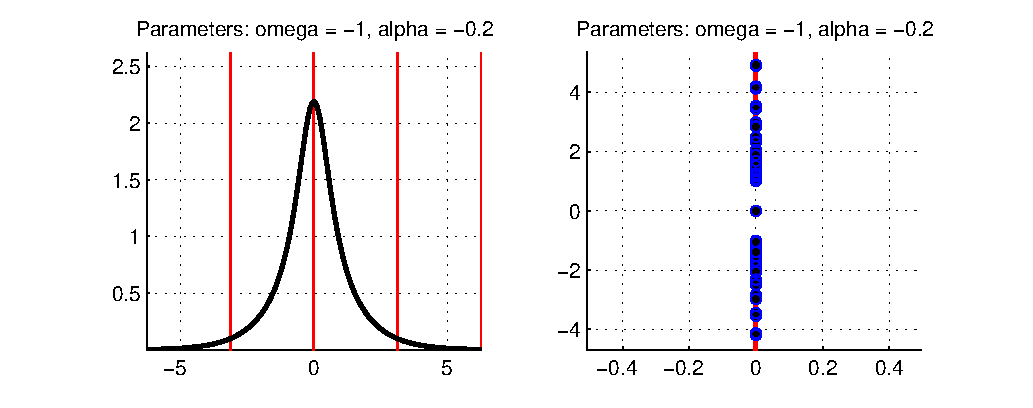
\includegraphics[width=1\linewidth]{pic/OA1O.eps} \ (A) $\{ \dots,O,A_1,O,\dots \}$}
	\end{minipage}
\hfill
	\begin{minipage}[h]{0.5\linewidth}
	\center{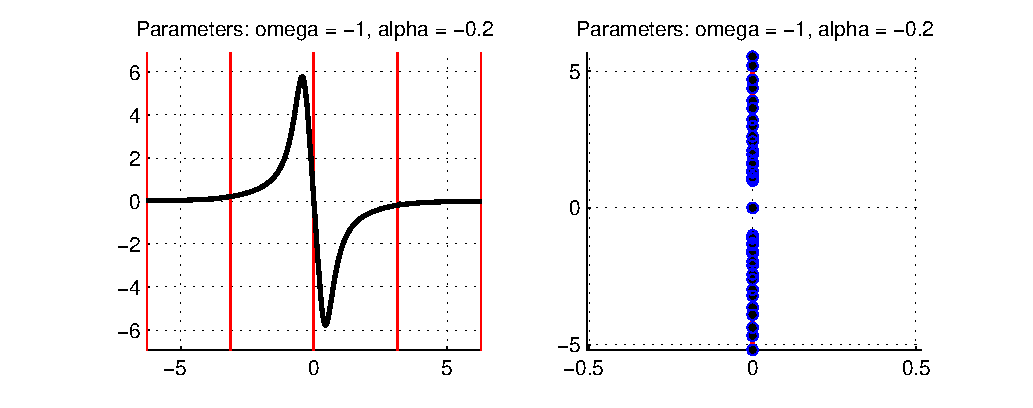
\includegraphics[width=1\linewidth]{pic/OB-1O.eps} \ (B) $\{ \dots,O,B_{-1},O,\dots \}$}
	\end{minipage}
\vfill
	\begin{minipage}[h]{0.5\linewidth}
	\center{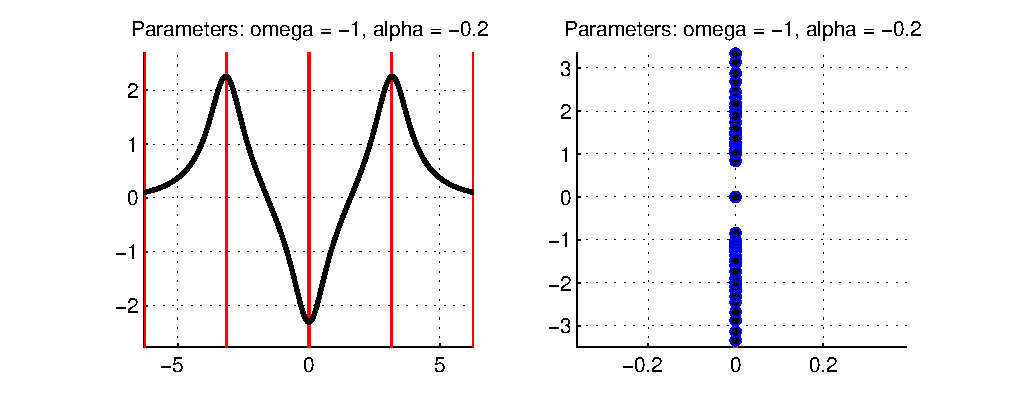
\includegraphics[width=1\linewidth]{pic/OA1A-1A1O.eps} \ (C) $\{ \dots,O,A_1,A_{-1},A_1,O,\dots \}$}
	\end{minipage}
\hfill
	\begin{minipage}[h]{0.5\linewidth}
	\center{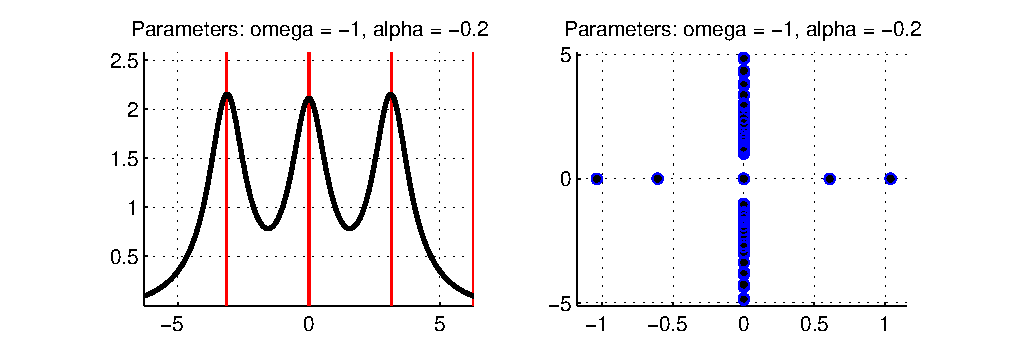
\includegraphics[width=1\linewidth]{pic/OA1A1A1O.eps} \ (D) $\{ \dots,O,A_1,A_1,A_1,O,\dots \}$}
	\end{minipage}
\vfill
	\begin{minipage}[h]{0.5\linewidth}
	\center{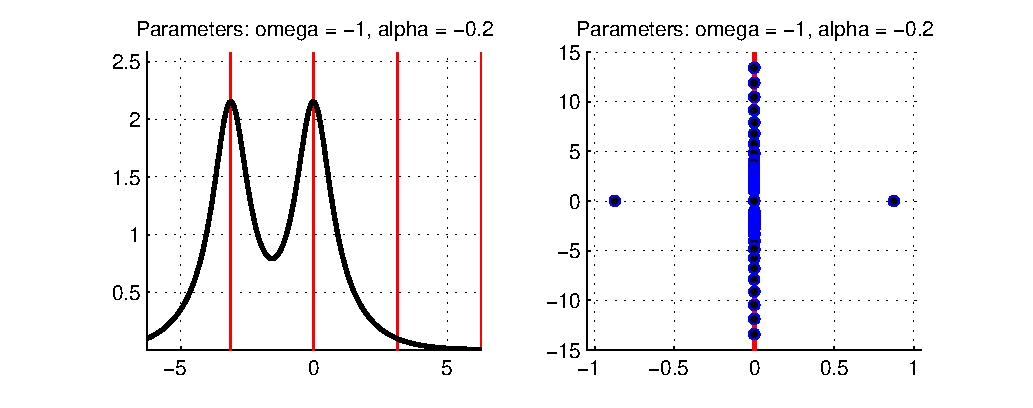
\includegraphics[width=1\linewidth]{pic/OA1A1O.eps} \ (E) $\{ \dots,O,A_1,A_1,O,\dots \}$}
	\end{minipage}
\hfill
	\begin{minipage}[h]{0.5\linewidth}
	\center{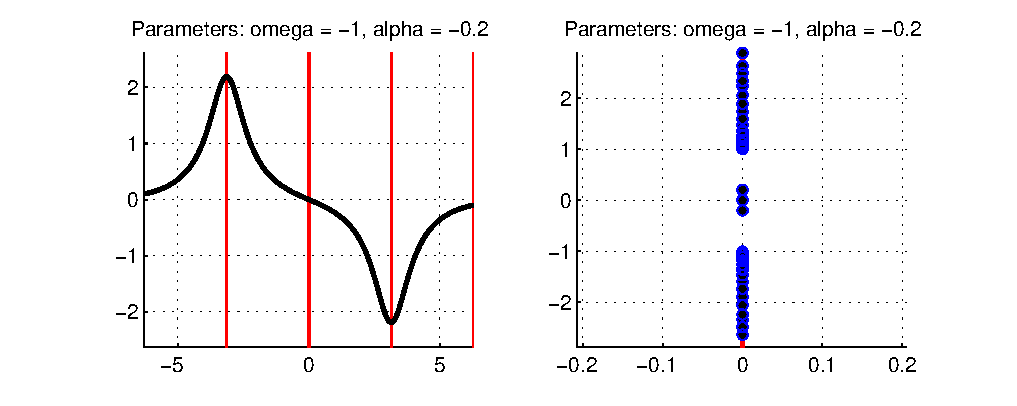
\includegraphics[width=1\linewidth]{pic/OA1OA-1O.eps} \ (F) $\{ \dots,O,A_1,O,A_{-1},O,\dots \}$}
	\end{minipage}
\vfill
	\begin{minipage}[h]{0.5\linewidth}
	\center{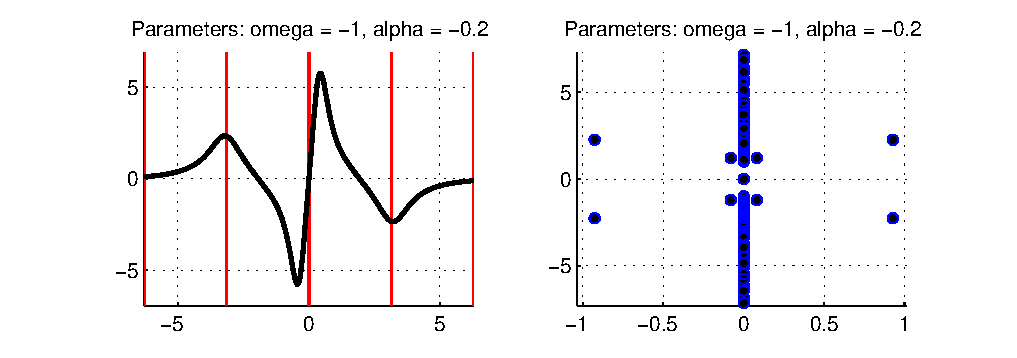
\includegraphics[width=1\linewidth]{pic/OA1B1A-1O.eps} \ (G) $\{ \dots,O,A_1,B_1,A_{-1},O,\dots \}$}
	\end{minipage}
\hfill
	\begin{minipage}[h]{0.5\linewidth}
	\center{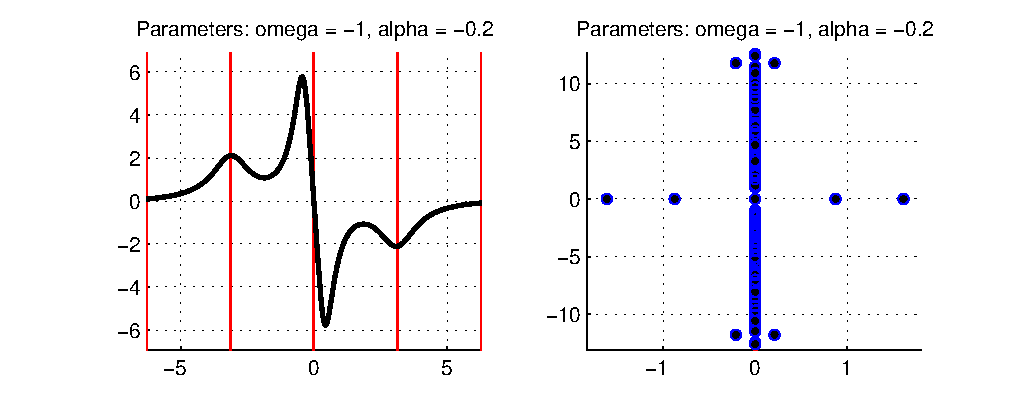
\includegraphics[width=1\linewidth]{pic/OA1B-1A-1O.eps} \ (H) $\{ \dots,O,A_1,B_{-1},A_{-1},O,\dots \}$}
	\end{minipage}
\caption{Локализованные решения, их коды и спектры линейной устойчивости соответствующих им операторов для значений параметров $\omega = -1$, $\alpha = -0.2$}
\label{pic:stability}
\end{figure}
%

Напомним, что в работе \cite{Malomed} была подробно исследована устойчивость FS решений как численно, так и аналитически, используя метод вариационной аппроксимации.
Существование в задаче (\ref{eq:stationary_obj}) устойчивого класса DS решений ранее не было известно и не обсуждалось в литературе.
Поэтому далее в этой главе мы подробно рассмотрим вопрос устойчивости дипольного солитона.

\section{DS: вариационная аппроксимация}

Некоторые общие свойства солитонных решений уравнения (\ref{eq:stationary_obj}) можно получить методом {\it вариационной аппроксимации} (ВА), принимая во внимание тот факт, что уравнение для стационарных состояний может быть получено из соответствующего лагранжиана
%
\begin{equation}
L = \int \limits_{-\infty}^{+\infty} \Big\{ \dfrac{1}{2} (u')^2 - \dfrac{1}{2} \omega u^2 - \dfrac{1}{4} [\alpha + \cos 2x] u^4 \Big\}.
\label{eq:lagrangian}
\end{equation}
%
В работе \cite{Malomed}, ВА была применена для анализа FS решений.
Для этого использовалась следующая подстановка:
%
\begin{equation}
u(x) = A \exp \left( -\dfrac{x^2}{2 W^2} \right),
\label{ea:fs_ansatz}
\end{equation}
%
отражающая тот факт, что FS решения имеют колоколообразную форму. 
В результате применения этого подхода, был предсказан факт наличия минимальной нормы FS решения
%
\begin{equation}
N \equiv \int \limits_{-\infty}^{+\infty} u^2(x) dx = \sqrt{\pi} A^2 W,
\end{equation}
%
а также существование порога устойчивости по амплитуде.

Аналогичное исследование для дипольного солитона (DS) произведем с помощью простейшей нечетной локализованной подстановки:
%
\begin{equation}
u(x) = Ax \exp \left( -\dfrac{x^2}{2 W^2} \right).
\label{eq:ds_ansatz}
\end{equation}
%
Максимальное значение $u(x)$, равное $\sqrt{e}AW$, достигается в $x_{max} = W$.
Следовательно параметр $W$ имеет значение полуширины дипольного солитона.
Норма соответствующей подстановки (\ref{eq:ds_ansatz}) равна
%
\begin{equation}
N = \dfrac{\sqrt{\pi}}{2} A^2 W^3.
\label{ds_norm}
\end{equation}
%
Уравнение (\ref{ds_norm}) позволяет выразить амплитуду через норму:
%
\begin{equation}
A^2 = \dfrac{2}{\sqrt{\pi}} \dfrac{N}{W^3}.
\label{eq:amplitude}
\end{equation}
% 
Подставляя соотношения (\ref{eq:ds_ansatz}), (\ref{eq:amplitude}) в лагранжиан (\ref{eq:lagrangian}) и, далее, интегрируя получившееся выражение, получаем следующее выражение для эффективного лагранжиана:
%
\begin{equation}
L_{\mathrm{eff}}=-\frac{\omega }{2}N+\frac{3N}{4W^{2}}-\frac{3\alpha N^{2}}{16\sqrt{2\pi}W}-\frac{N^{2}e^{-W^{2}/2}}{16\sqrt{2\pi}W}\left(3-6W^{2}+W^{4}\right).
\label{eq:lagrangian_eff}
\end{equation}
%
Вариационные уравнения Эйлера-Лагранжа для эффективного лагранжиана (\ref{eq:lagrangian_eff}) имеют вид
%
\begin{eqnarray}
\partial L_{\mathrm{eff}}/\partial W = 0; \label{eq:dw} \\
\partial L_{\mathrm{eff}}/\partial N = 0, \label{eq:dn}
\end{eqnarray}
%
где $W$ и $N$ --- свободные вариационные параметры для заданного $\omega$.

Далее, вслед за авторами работы \cite{Malomed}, рассматривается случай $\alpha = 0$.
Уравнение (\ref{eq:dw}) позволяет получить связь величин $N$ и $W$ вида:
%
\begin{equation}
N=\frac{48\sqrt{\pi /2}\exp \left( W^{2}/2\right) }{W\left(3+9W^{2}-9W^{4}+W^{6}\right) }.
\label{eq:N(W)}
\end{equation}
%
Это соотношение изображено на Рис. \ref{pic:N(W)}.
%
\begin{figure}
\center{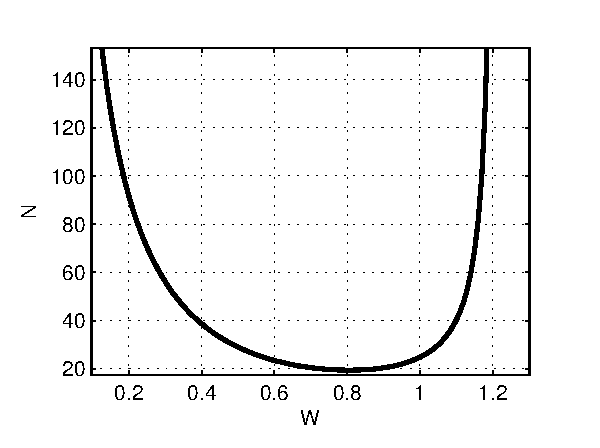
\includegraphics[width=0.5\textwidth]{pic/N(W).eps}}
\caption{Соотношение между нормой и полушириной дипольного солитона, предсказываемое вариационной аппроксимацией, $\alpha = 0$}
\label{pic:N(W)}
\end{figure}
%
Минимальное значение нормы дипольного солитона, предсказываемое вариационной аппроксимацией, достигается при значении $W = W_0 \approx 0.806$ и равно
%
\begin{equation}
N_{\mathrm{min}}^{\mathrm{(VA)}} \approx 19.41
\label{eq:norm_min_va}
\end{equation}
%

Таким образом, вариационная аппроксимация предсказывает существование минимальной нормы, при которой существует дипольный солитон.
В терминах БЭК это означает, что дипольный солитон не наблюдается при малом количестве частиц, образующих конденсат.
Более того, из соотношения (\ref{eq:N(W)}) следует, что величина $W$ может изменять лишь в конечных пределах:
%
\begin{equation}
0 < W < W_{\mathrm{max}} \approx 1.21.
\end{equation}
%

Второе вариационное уравнений (\ref{eq:dn}) после некоторых преобразований обнаруживает монотонную зависимость между $\omega$ и $W$ вида
%
\begin{equation}
\omega =\frac{3}{2}\frac{-9+33W^{2}-13W^{4}+W^{6}}{W^{2}\left( 3+9W^{2}-9W^{4}+W^{6}\right) }.
\label{eq:omega}
\end{equation}
%
Объединяя это с соотношением (\ref{eq:N(W)}), применим критерий устойчивости Вахитова-Колоколова \cite{JYang}; $dN / d\omega \equiv (d\omega / dW)^{-1} dN / dW < 0$.
Из выражения (\ref{eq:omega}) следует, что величина $d\omega / dW$ всегда положительна.
Критерий Вахитова-Колоколова предсказывает устойчивость левой ветки решений типа DS на Рис. \ref{pic:N(W)}, где $dN / dW < 0$, что соответствует интервалу значений $W$
%
\begin{equation}
0 < W < W_0 \approx 0.806,
\end{equation}
%
в то время как правая ветка, $dN / dW > 0$, т.е. $W > W_0$ оказывается неустойчивой.
Стоит отметить, что сам метод вариационной аппроксимации дает крайне приближенные значение количественных характеристик в силу неточности метода, однако качественные предсказания оказываются весьма полезными.
Подведем итоги применения вариационной аппроксимации к классу решений типа DS.
Вариационная аппроксимация предсказывает, что
%
\begin{itemize}
\item[(a)] существует минимальная норма дипольного солитона;
\item[(б)] существует максимально возможная ширина дипольного солитона;
\item[(в)] существует граница по ширине DS, которая отделяет устойчивую ветку решений от неустойчивой.
\end{itemize}
%
В следующих разделах мы покажем, что все эти предсказания качественно согласуются с результатами численного эксперимента.

\section{DS: численное исследование}

Численное исследование семейства DS решений производилось численно с помощью метода стрельбы.
В этом разделе представлены основные результаты этого исследования.

Семейство DS решений может быть запараметризовано с помощью $\omega$ или же с помощью параметра $W$, который в нашем случае определен как расстояние от центральной точки до точки максимума DS солитона и имеет смысл полуширины дипольного солитона.
Было обнаружено, что амплитуда и норма растут при уменьшении характерной ширины солитона, т.е. когда $W$ стремиться к нулю, а $\omega$ стремиться к $-\infty$.
Примеры различных профилей изображены на Рис. \ref{pic:dss}
%
\begin{figure}
\center{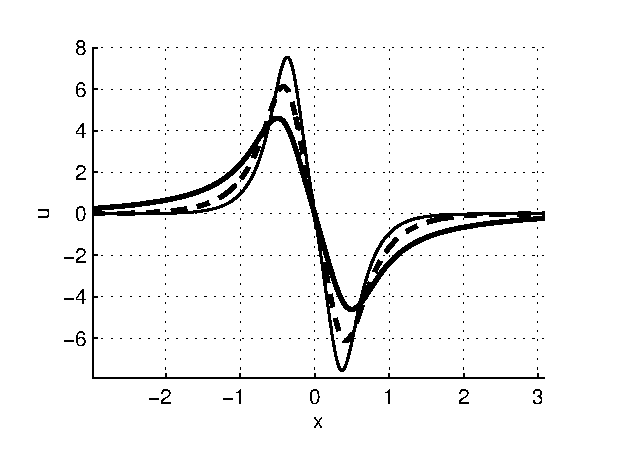
\includegraphics[width=0.5\textwidth]{pic/DSs.eps}}
\caption{Численно построенные профили дипольных солитонов при значениях $\omega = -15$ (тонкая линия), $\omega = -7$ (пунктирная линия) и $\omega = -1$ (толстая линия) для $\alpha = 0$}
\label{pic:dss}
\end{figure}
%

Численно определенное соотношение нормы $N$ и полуширины $W$ изображено на Рис. \ref{pic:N(W)_numerical}.
Из этого графика видно, что существует минимальная норма, необходимая для существования дипольного солитона, как это и было предсказано с помощью вариационной аппроксимации (пункт (а)).
%
\begin{figure}
\center{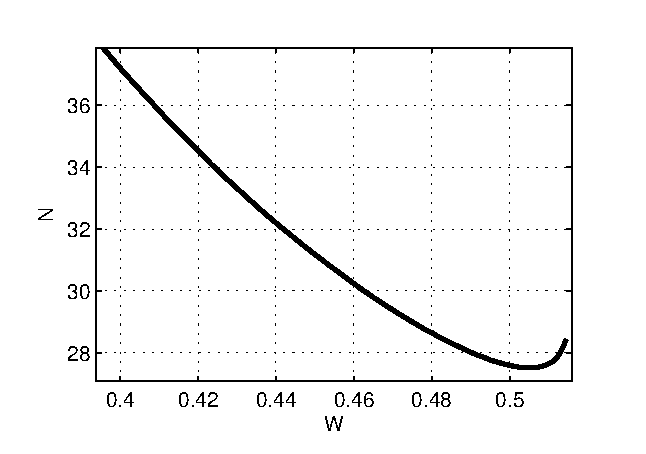
\includegraphics[width=0.5\textwidth]{pic/N(W)_numerical.eps}}
\caption{Численно построенная зависимость $N(W)$, нормы от полуширины дипольного солитона для $\alpha = 0$}
\label{pic:N(W)_numerical}
\end{figure}
%

С помощью численного счета было показано, что дипольный солитон, имеющий код $\{ \dots, O, B_{\pm 1}, O, \dots \}$, существует при $\omega < \omega^*$, где $\omega^* = 0.2654$.
В точке $\omega^*$ он претерпевает бифуркацию типа седло-узел и пропадает вместе с веткой решения, отвечающей коду $\{ \dots, O, A_{\mp 1}, B_{\pm 1}, A_{\pm 1}, O, \dots \}$.
Соответствующая бифуркационная диаграмма изображена на Рис. \ref{pic:bifurcation}.
Это означает, что ширина (полуширина $W$) ограничена сверху, как это и предсказывалось вариационной аппроксимацией (пункт (б)).

Таким образом результаты вариационной аппроксимации качественно согласуются с численным счетом, хотя точность такой аппроксимации недостаточна.
Например, минимальная норма, предсказанная с помощью ВА, оказывается на $30\%$ меньше численно полученного значения $N_{\mathrm{min}}^{\mathrm{(num)}} \approx 27.5$.
%
\begin{figure}
\center{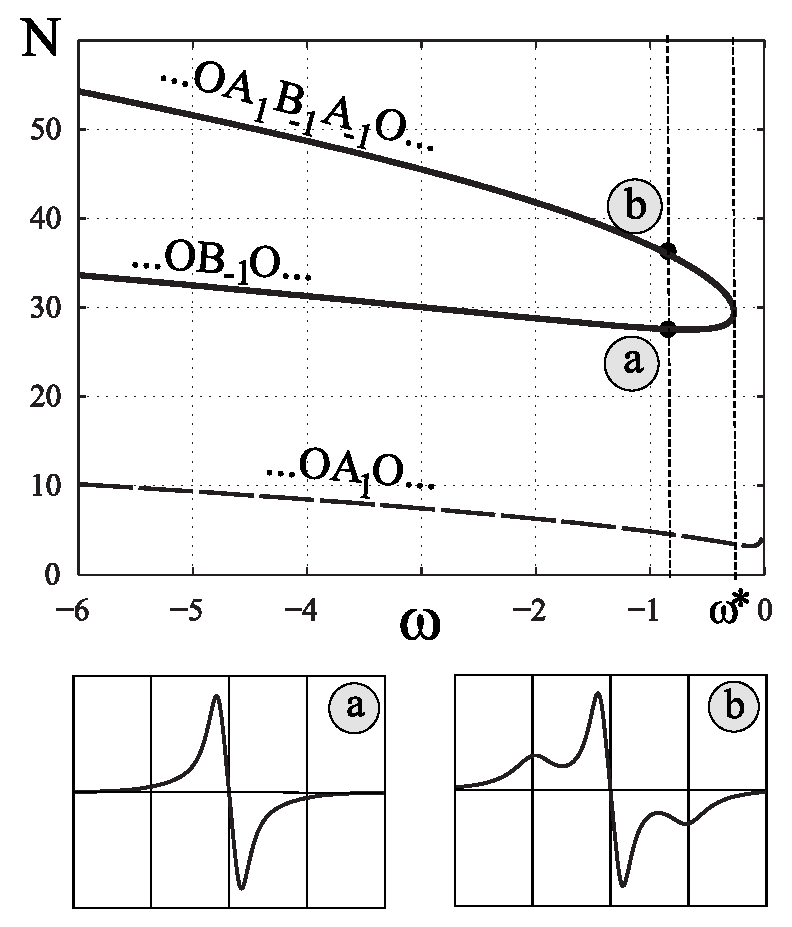
\includegraphics[width=0.5\textwidth]{pic/bifurcation.eps}}
\caption{Бифуркационная диаграмма при $\alpha = 0$: ветка решения типа DS, отвечающая коду $\{ \dots, O, B_{\pm 1}, O, \dots \}$ претерпевает бифуркацию и пропадает вместе с веткой решения, отвечающей коду $\{ \dots, O, A_{\mp 1}, B_{\pm 1}, A_{\pm 1}, O, \dots \}$. Два профиля соответствующих решений построены для значения $\omega = -0.8$.}
\label{pic:bifurcation}
\end{figure}
%

\section{DS: эволюционное моделирование}

С целью проверки предположения (в), полученного в результате применения вариационной аппроксимации, было произведено моделирование эволюции дипольного солитона во времени.
Для этого была использована консервативная конечно-разностная схема Трофимова-Пескова \cite{Trofimov}.
Эта схема замечательна тем, что сохраняет норму решения (\ref{eq:norm}) и значение функционала энергии (\ref{eq:energy}).
Она является неявной, однако позволяет проводить расчеты с большим временным шагом.
Для устранения эффекта отражения от концов был использован прием искусственной диссипации на краях.
С целью выявления неустойчивости стационарной моды, она возмущалась некоторым малым пространственным возмущением.
В расчетах использовалась конечная пространственная область $[-4\pi, 4\pi]$.

Некоторые результаты моделирования представлены на Рис. \ref{pic:evolution_unst}, \ref{pic:evolution_st}.
В случае, когда дипольный солитон оказывается неустойчивым, он перестраивается в устойчивый фундаментальный солитон.
Этот факт отражен на Рис. \ref{pic:evolution_unst} и Рис. \ref{pic:summary}.
Численный эксперимент позволяет заключить, что предсказание (в), полученное в результате вариационной аппроксимации, также верно.
Результаты моделирования удобно изобразить на графике $N(\omega)$, Рис. \ref{pic:summary}.
Левая ветка решения, где наклон графика $N(\omega)$ отрицателен, демонстрирует устойчивое поведение, в то время как правая ветка (наклон графика $N(\omega)$ положителен) неустойчива.
Этот факт согласуется с результатами вариационной аппроксимации и критерием Вахитова-Колоколова.
Однако точная граница между устойчивой и неустойчивой областью осталась неясна.
Это связано с тем, что для параметров $\omega$ вблизи минимума графика $N(\omega)$ эволюция дипольного солитона зависит от типа возмущения и параметров численного счета.
%
\begin{figure}
	\center{\begin{minipage}[h]{0.75\linewidth}
	\center{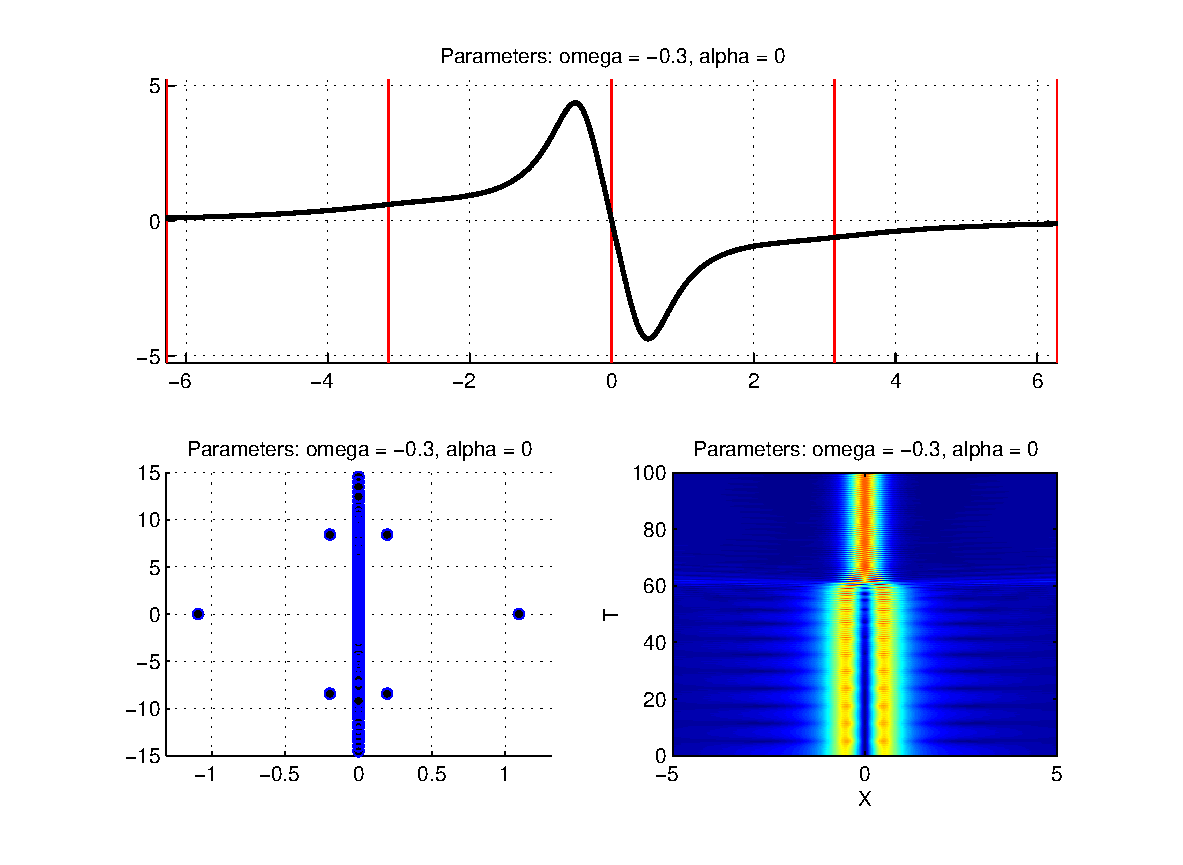
\includegraphics[width=1\linewidth]{pic/omega=-03alpha=0.eps} \ (A) $\omega = -0.3$}
	\end{minipage}}
	\center{\begin{minipage}[h]{0.75\linewidth}
	\center{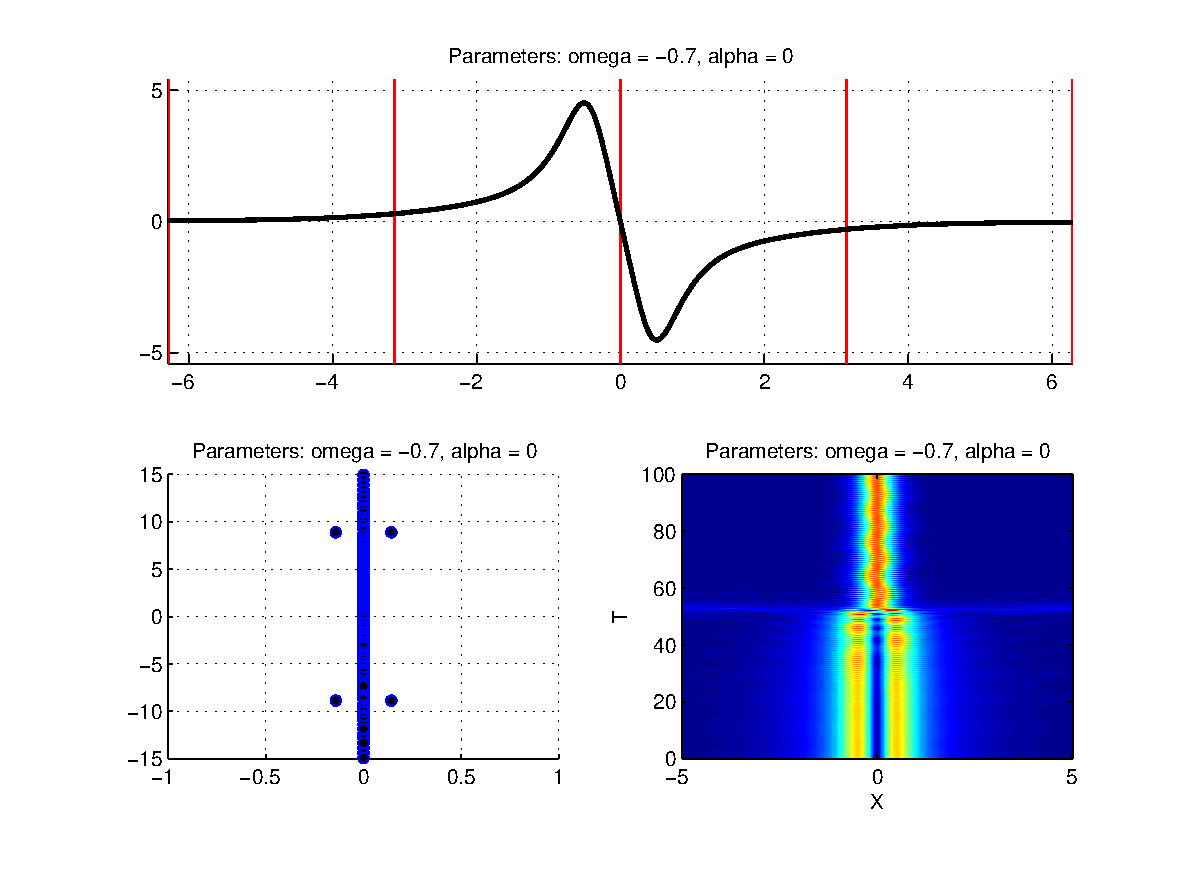
\includegraphics[width=1\linewidth]{pic/omega=-07alpha=0.eps} \ (B) $\omega = -0.7$}
	\end{minipage}}
\caption{Эволюция неустойчивых дипольных солитонов и соответствующие им спектры при $\alpha = 0$.}
\label{pic:evolution_unst}
\end{figure}
%
\begin{figure}
	\center{\begin{minipage}[h]{0.75\linewidth}
	\center{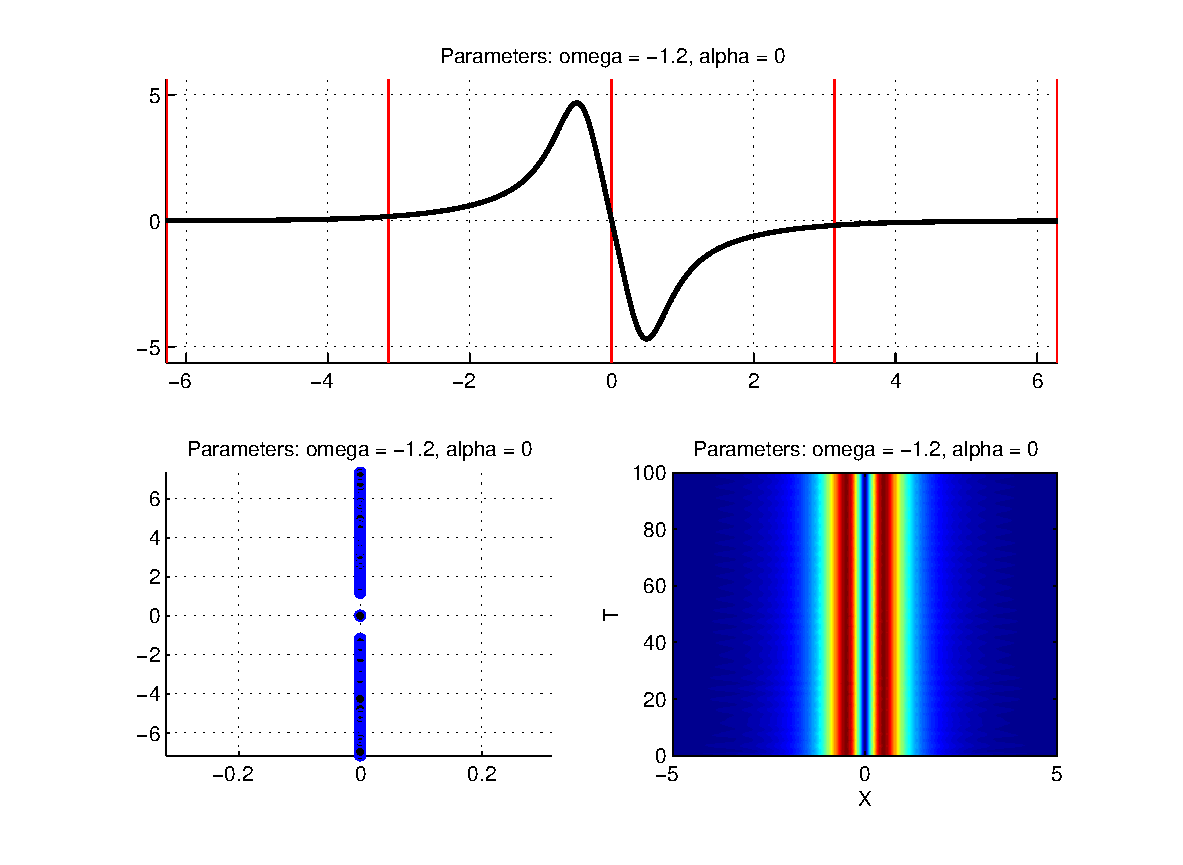
\includegraphics[width=1\linewidth]{pic/omega=-12alpha=0.eps} \ (A) $\omega = -1.2$}
	\end{minipage}}
	\center{\begin{minipage}[h]{0.75\linewidth}
	\center{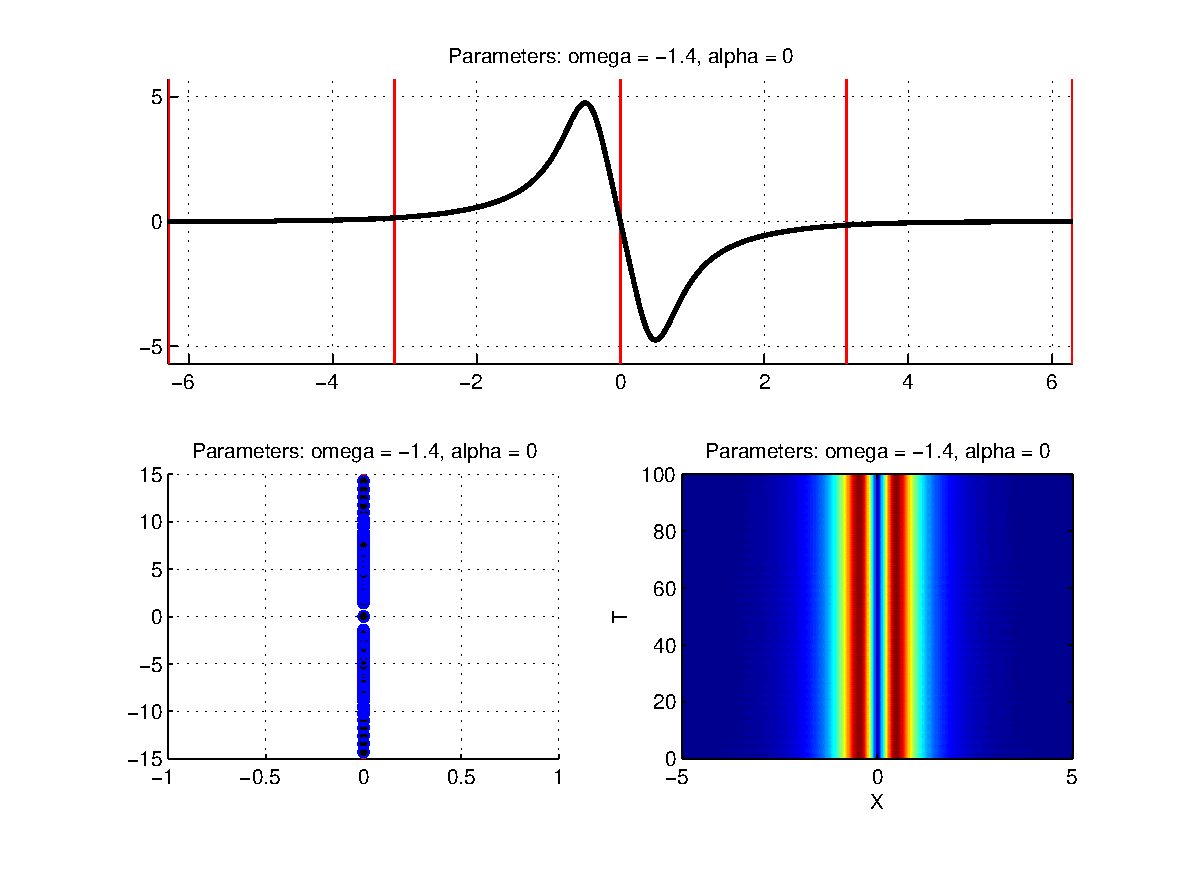
\includegraphics[width=1\linewidth]{pic/omega=-14alpha=0.eps} \ (B) $\omega = -1.4$}
	\end{minipage}}
\caption{Эволюция устойчивых дипольных солитонов и соответствующие им спектры при $\alpha = 0$.}
\label{pic:evolution_st}
\end{figure}
%
\begin{figure}
\center{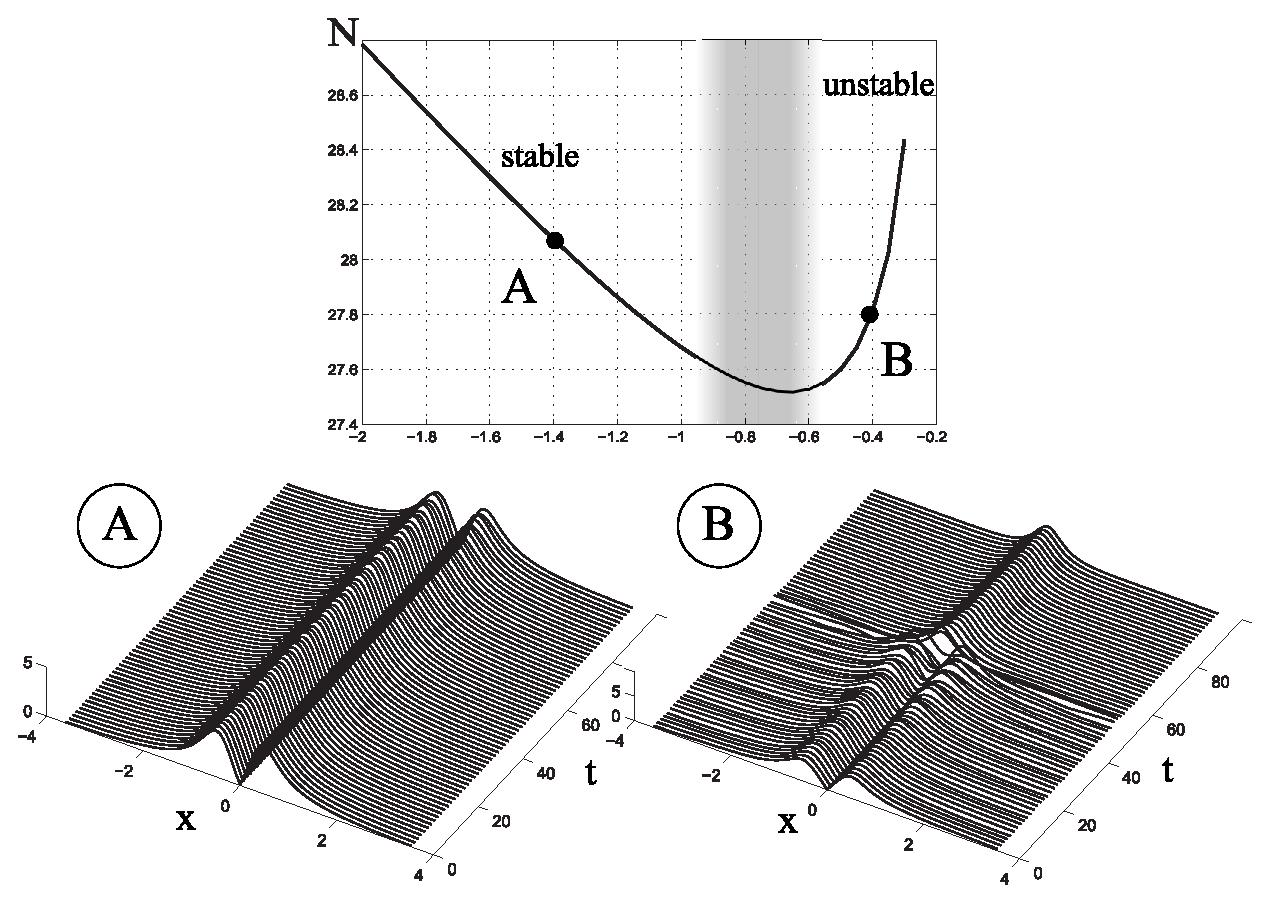
\includegraphics[width=0.8\textwidth]{pic/summary.eps}}
\caption{Численно построенная зависимость $N(\omega)$ при $\alpha = 0$; (A) устойчивый дипольный солитон, $\omega = -1.4$; (B) неустойчивый дипольный солитон, $\omega = -0.4$, в ходе эволюции превращается в устойчивый фундаментальный солитон с параметрами $\omega \approx -13.96$ и амплитудой $\approx 5.43$.}
\label{pic:summary}
\end{figure}
%

\conclusion

\bibliographystyle{gost2008}
\bibliography{biblio}

\end{document}